\documentclass[letter,12pt]{article}
\usepackage[paperheight=27.94cm,paperwidth=21.59cm,bindingoffset=0in,left=3cm,right=2.0cm, top=3.5cm,bottom=2.5cm, headheight=200pt, headsep=1.0\baselineskip]{geometry}
\usepackage{graphicx,lastpage}
\usepackage{upgreek}
\usepackage{censor}
\usepackage[spanish,es-tabla]{babel}
\usepackage{pdfpages}
\usepackage{tabularx}
\usepackage{graphicx}
\usepackage{adjustbox}
\usepackage{xcolor}
\usepackage{colortbl}
\usepackage{rotating}
\usepackage{multirow}
\usepackage[utf8]{inputenc}
\usepackage{float}
\usepackage{hyperref}
\usepackage{listings}

\renewcommand{\tablename}{Tabla}
\usepackage{fancyhdr}
\pagestyle{fancy}

\fancyhead[L]{}
%
\begin{document}
%
   \title{\Huge{Informe Laboratorio 2}}

      \author{\textbf{Sección 3} \\  \\Nicolás Gutiérrez \\ e-mail: nicolas.gutierrez6@mail.udp.cl}
          
   \date{Septiembre de 2026}

   \maketitle
   
   \tableofcontents
 
  \newpage
  

\section{Descripción de actividades}
Utilizando la aplicación web vulnerable DVWA

(Damn Vulnerable Web App - \href{https://github.com/digininja/DVWA}{https://github.com/digininja/DVWA} (Enlaces a un sitio externo.)) realice las siguientes actividades:


\begin{itemize}
    \item Despliegue la aplicación en su equipo utilizando docker. Detalle el procedimiento y explique los parámetros que utilizó.
    \item Utilice Burpsuite (https://portswigger.net/burp/communitydownload (Enlaces a un sitio externo.)) para realizar un ataque de fuerza bruta contra formulario ubicado en vulnerabilities/brute. Explique el proceso y obtenga al menos 2 pares de usuario/contraseña válidos. Muestre las diferencias observadas en burpsuite.
    \item Utilice la herramienta cURL, a partir del código obtenido de inspect elements de su navegador, para realizar un acceso válido y uno inválido al formulario ubicado en vulnerabilities/brute. Indique 4 diferencias entre la página que retorna el acceso válido y la página que retorna un acceso inválido.
    \item Utilice la herramienta Hydra para realizar un ataque de fuerza bruta contra formulario ubicado en vulnerabilities/brute. Explique el proceso y obtenga al menos 2 pares de usuario/contraseña válidos.
    \item Compare los paquetes generados por hydra, burpsuite y cURL. ¿Qué diferencias encontró? ¿Hay forma de detectar a qué herramienta corresponde cada paquete?

    \item Desarrolle un script en Python para realizar un ataque de fuerza bruta:

    \begin{itemize}
        \item Utilice la librería requests para interactuar con el formulario ubicado en vulnerabilities/brute y desarrollar su propio script de fuerza bruta en Python.
        El script debe realizar intentos de inicio de sesión probando una lista de combinaciones de usuario/contraseña.

        \item  Identifique y explique la cabecera HTTP que empleará para realizar el ataque de fuerza bruta.

        \item  Muestre el código y los resultados obtenidos (al menos 2 combinaciones válidas de usuario/contraseña).

        \item Compare el rendimiento de este script en Python con las herramientas Hydra, Burpsuite, y cURL en términos de velocidad y detección.
    \end{itemize}

    \item  Investigue y describa 4 métodos comunes para prevenir o mitigar ataques de fuerza bruta en aplicaciones web:

    \begin{itemize}
        \item Para cada método, explique su funcionamiento, destacando en qué escenarios es más eficaz.

    \end{itemize}


    
\end{itemize}

\section{Desarrollo de actividades según criterio de rúbrica}

\subsection{Levantamiento de docker para correr DVWA (dvwa)}
Para obtener la imagen de la aplicación web vulnerable DVWA, se ejecutó el comando \textbf{\texttt{docker pull vulnerables/web-dvwa}}. Este comando descarga desde Docker Hub la versión más reciente de la imagen del contenedor con sus dependencias (servidor Apache, PHP y base de datos). Para comprobar que la imagen se descargó e instaló correctamente en el almacenamiento local, se utilizó el comando \textbf{\texttt{docker images}}, tal como se observa en la Figura~\ref{fig:docker_pull}.

\begin{figure}[H]
    \centering
    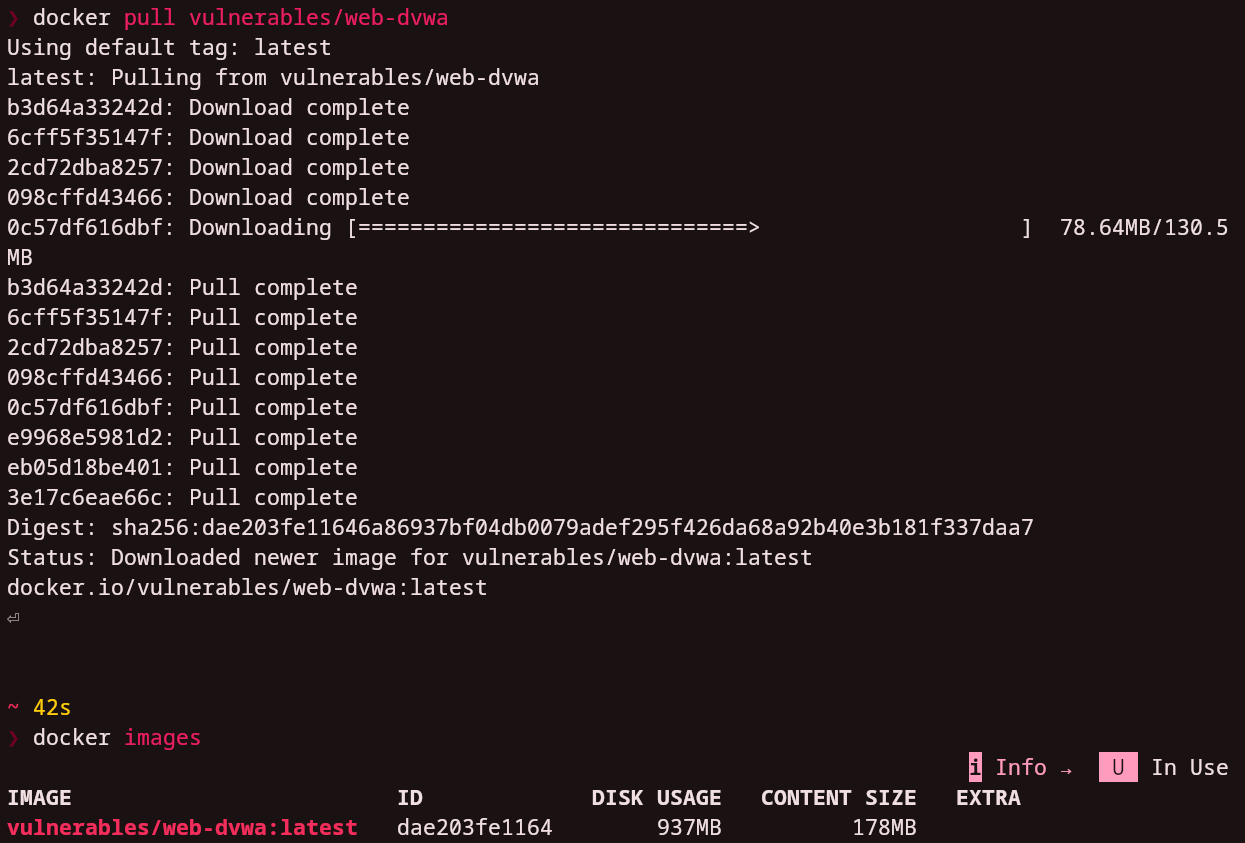
\includegraphics[width=0.9\linewidth]{imagenes/EvidenciaDokerPull.png}
    \caption{Evidencia de descarga y verificación de la imagen de DVWA.}
    \label{fig:docker_pull}
\end{figure}

\subsection{Redirección de puertos en docker (dvwa)}
Para desplegar el contenedor e interactuar con la aplicación desde el navegador anfitrión, se ejecutó el comando \textbf{\texttt{docker run -d --name dvwa\_lab -p 8080:80 vulnerables/web-dvwa}}. En la Figura~\ref{fig:docker_ports} se evidencia el estado activo del contenedor y la redirección exitosa de puertos obtenida mediante el comando \textbf{\texttt{docker ps}}.

A continuación, se detalla la función de cada parámetro utilizado en la instrucción:
\begin{itemize}
    \item \textbf{\texttt{-d}} (\textit{detached}): Ejecuta el contenedor en segundo plano, liberando la terminal para seguir ingresando comandos.
    \item \textbf{\texttt{--name dvwa\_lab}}: Asigna el nombre personalizado \texttt{dvwa\_lab} al contenedor para facilitar su identificación y administración.
    \item \textbf{\texttt{-p 8080:80}}: Realiza el mapeo de puertos (\textit{port forwarding}), enlazando el puerto \texttt{8080} de la máquina anfitriona con el puerto \texttt{80} interno del contenedor donde escucha el servidor web.
\end{itemize}

\begin{figure}[H]
    \centering
    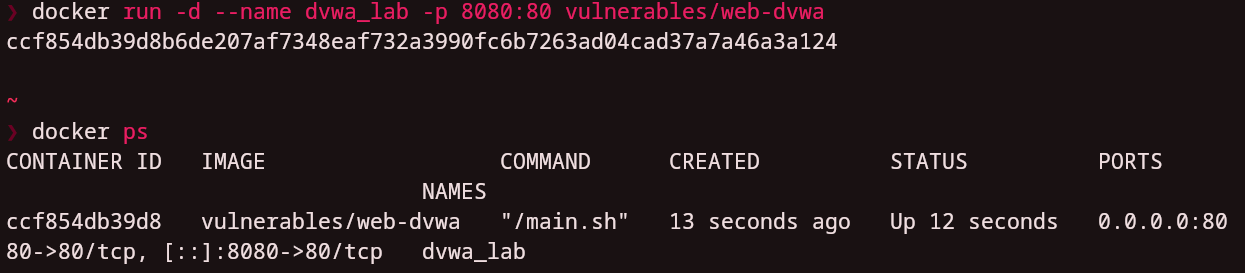
\includegraphics[width=0.9\linewidth]{imagenes/EvidenciaRedireccionDePuertos.png}
    \caption{Evidencia de ejecución del contenedor y redirección de puertos de DVWA.}
    \label{fig:docker_ports}
\end{figure}
\subsection{Obtención de consulta a replicar (burp)}

Para capturar la consulta HTTP que será replicada durante el ataque, se configuró el navegador para redirigir el tráfico a través del proxy de Burp Suite. A continuación, se accedió al módulo \texttt{vulnerabilities/brute} y se envió un intento de inicio de sesión con credenciales de prueba.

Como se observa en la Figura~\ref{fig:burp_request}, Burp Suite interceptó exitosamente la petición HTTP \texttt{GET}, capturando la URI de destino, los parámetros de autenticación (\texttt{username}, \texttt{password} y \texttt{Login}) y las cabeceras requeridas, como la cookie de sesión (\texttt{PHPSESSID}) y el nivel de seguridad. Esta consulta capturada sirve como la estructura base que se enviará a la herramienta \textit{Intruder} para automatizar el ataque.

\begin{figure}[H]
    \centering
    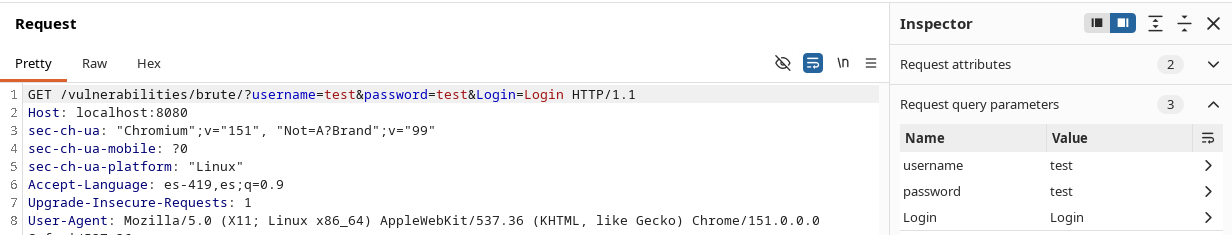
\includegraphics[width=0.9\textwidth]{imagenes/PeticiónHTTPGETCapturadaEnBurpSuite.png} 
    \caption{Petición HTTP GET capturada en Burp Suite para la sección de fuerza bruta.}
    \label{fig:burp_request}
\end{figure}

\newpage

\subsection{Identificación de campos a modificar (burp)}

Una vez capturada la consulta en el proxy, se envió la petición a la herramienta \textit{Intruder} (utilizando la combinación de teclas \texttt{Ctrl + I}) para configurar el ataque automatizado. En el módulo \textit{Intruder}, se ingresó a la pestaña \textbf{Positions} para identificar y delimitar las variables de la consulta HTTP que serán modificadas dinámicamente durante el ataque de fuerza bruta.

Al inspeccionar la estructura de la URI en la petición \texttt{GET}, se identificaron los parámetros de consulta que reciben los datos enviados por el usuario:
\begin{itemize}
    \item \textbf{\texttt{username}}: Parámetro encargado de transmitir el nombre de usuario.
    \item \textbf{\texttt{password}}: Parámetro encargado de transmitir la contraseña.
    \item \textbf{\texttt{Login}}: Parámetro de acción que activa la validación del formulario en el servidor.
\end{itemize}

Para definir las posiciones de inyección, se limpiaron los marcadores automáticos con el botón \textbf{Clear \S} y se establecieron manualmente los símbolos de delimitación (\texttt{\S}) rodeando únicamente los valores de los campos \texttt{username} y \texttt{password}, tal como se observa en la Figura~\ref{fig:burp_positions}. Adicionalmente, se seleccionó el tipo de ataque \textbf{Cluster Bomb}, el cual permite utilizar dos conjuntos independientes de diccionarios e iterar todas las combinaciones posibles entre usuarios y contraseñas.

\begin{figure}[H]
    \centering
    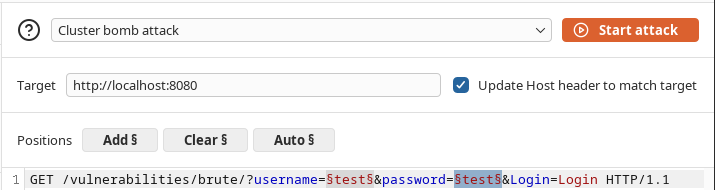
\includegraphics[width=0.9\linewidth]{imagenes/EvidenciaCamposBurp.png}
    \caption{Identificación y delimitación de los campos \texttt{username} y \texttt{password} con ataque \textit{Cluster Bomb} en Burp Suite Intruder.}
    \label{fig:burp_positions}
\end{figure}

\newpage

\subsection{Obtención de diccionarios para el ataque (burp)}

Para ejecutar el ataque de fuerza bruta mediante el método \textit{Cluster Bomb}, es necesario configurar diccionarios de palabras independientes para cada una de las posiciones definidas en la petición HTTP. En la pestaña \textbf{Payloads} de Burp Suite Intruder, se procedió a cargar y configurar las listas de prueba para las variables de autenticación.

Para el primer conjunto de datos (\textbf{Payload position 1}, correspondiente al parámetro \texttt{username}), se utilizó el tipo de payload \textbf{Simple list} y se cargó una lista de nombres de usuario comunes mediante el panel de configuración, como se evidencia en la Figura~\ref{fig:burp_payloads}. De igual manera, se configuró el segundo conjunto (\textbf{Payload position 2}, correspondiente al parámetro \texttt{password}) cargando el diccionario de contraseñas de prueba. Esta configuración genera el total de combinaciones necesarias para iterar y evaluar las respuestas del servidor.

\begin{figure}[H]
    \centering
    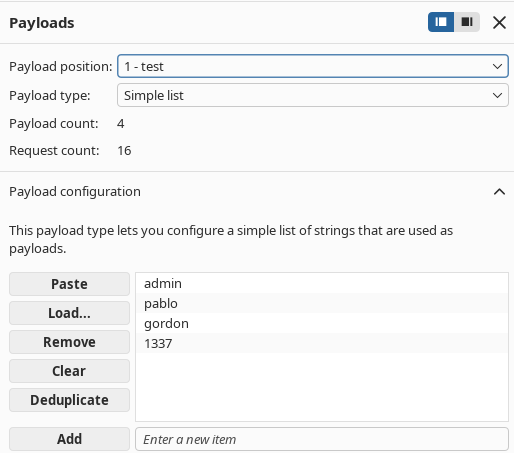
\includegraphics[width=0.7\linewidth]{imagenes/EvidenciaDiccionariosBurp.png}
    \caption{Configuración del diccionario de palabras para la posición de usuarios en Burp Suite Intruder.}
    \label{fig:burp_payloads}
\end{figure}

\newpage

\subsection{Obtención de al menos 2 pares (burp)}

Una vez configuradas las posiciones e inyectados los diccionarios en la herramienta \textit{Intruder}, se inició el ataque automatizado presionando el botón \textbf{Start attack}. Al finalizar la ejecución de las peticiones, se procedió a analizar la tabla de resultados para discriminar entre los intentos de inicio de sesión fallidos y los accesos exitosos.

Debido a que el servidor web devuelve un código de estado \texttt{HTTP 200 OK} tanto para peticiones válidas como inválidas, el parámetro diferenciador primario es la columna \textbf{Length} (longitud de la respuesta HTTP en bytes). Al ordenar las peticiones por esta columna, se observó que los intentos fallidos mantienen una longitud uniforme de 4,703 o 4,702 bytes, correspondiente a la estructura que renderiza el mensaje de error \texttt{Username and/or password incorrect}. Por el contrario, los intentos con credenciales correctas presentan una longitud de respuesta mayor (4,740 y 4,741 bytes).

Al inspeccionar el cuerpo de la respuesta en los paquetes con longitud divergente, se confirmó el acceso exitoso mediante la presencia del mensaje \texttt{Welcome to the password protected area}, tal como se aprecia en la Figura~\ref{fig:burp_results}. De este modo, se obtuvieron exitosamente los siguientes dos pares válidos de usuario y contraseña:
\begin{itemize}
    \item \textbf{Par 1:} \texttt{admin} : \texttt{password}
    \item \textbf{Par 2:} \texttt{pablo} : \texttt{letmein}
\end{itemize}

\begin{figure}[H]
    \centering
    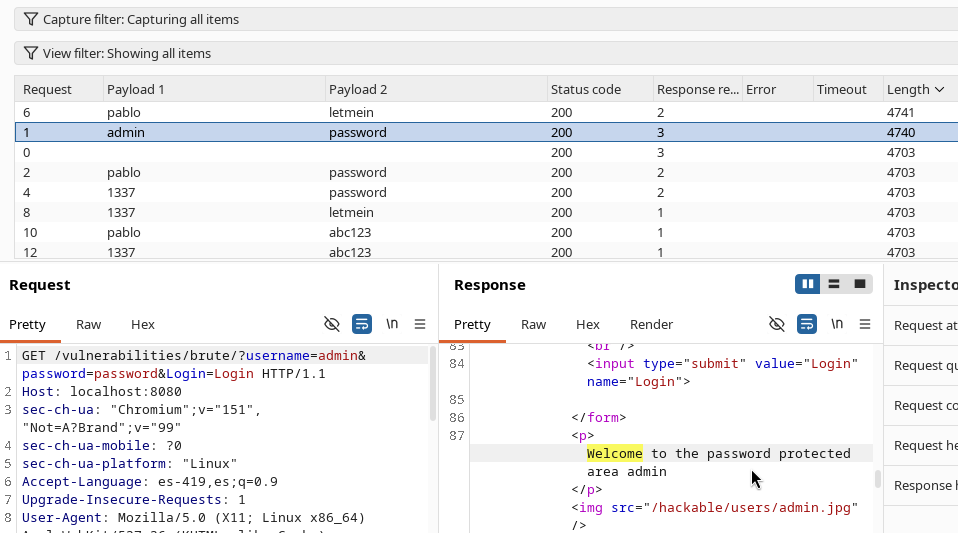
\includegraphics[width=0.9\linewidth]{imagenes/EvidenciaDosParesBurp.png}
    \caption{Resultados del ataque de fuerza bruta en Burp Suite Intruder ordenados por la columna \textit{Length}, resaltando los pares válidos obtenidos y la confirmación en la respuesta HTML.}
    \label{fig:burp_results}
\end{figure}

\subsection{Obtención de código de inspect element (curl)}

Para analizar e interactuar con la aplicación utilizando herramientas de línea de comandos, se procedió a exportar la solicitud HTTP de inicio de sesión directamente desde el navegador. Para ello, se accedió al módulo \texttt{vulnerabilities/brute} en DVWA y se abrieron las herramientas de desarrollo (\textit{DevTools}) mediante la tecla \texttt{F12}.

Tras enviar un intento de autenticación en el formulario, se seleccionó la pestaña \textbf{Red} (\textit{Network}) y se localizó la petición HTTP \texttt{GET} dirigida a la ruta del desafío. Haciendo clic derecho sobre la solicitud, se seleccionó la opción \textbf{Copiar valor} $\rightarrow$ \textbf{Copiar como cURL}, tal como se ilustra en la Figura~\ref{fig:copy_curl}. 

Este procedimiento permite obtener la estructura exacta de la instrucción de consola \texttt{cURL}, incluyendo la URI de destino, los parámetros enviádos por el formulario y las cabeceras HTTP requeridas para mantener la sesión activa, tales como las cookies \texttt{PHPSESSID} y \texttt{security=low}.

\begin{figure}[H]
    \centering
    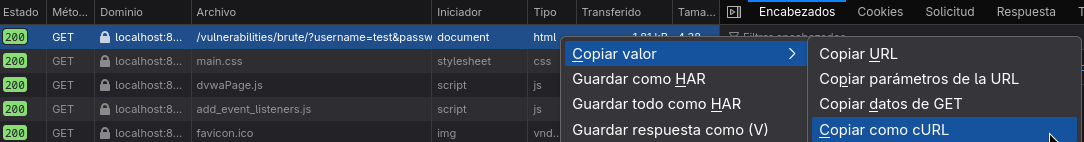
\includegraphics[width=0.9\linewidth]{imagenes/EvidenciaCopyCurl.png}
    \caption{Exportación de la petición HTTP desde las herramientas de desarrollo del navegador utilizando la opción \textit{Copiar como cURL}.}
    \label{fig:copy_curl}
\end{figure}

\subsection{Utilización de curl por terminal (curl)}

A partir de la solicitud exportada desde el navegador, se procedió a ejecutar las peticiones HTTP en la terminal mediante la herramienta \texttt{cURL}. Para analizar e inspeccionar las respuestas del servidor de forma legible, se incluyó el parámetro \texttt{-i} junto con un filtro de salida para obtener las cabeceras de estado y las líneas clave del cuerpo HTML.

Se realizaron dos ejecuciones manteniendo activa la sesión autenticada mediante la cabecera de cookies (\texttt{PHPSESSID}):
\begin{enumerate}
    \item \textbf{Acceso Válido:} Se envió una solicitud con credenciales correctas (\texttt{username=admin} y \texttt{password=password}).
    \item \textbf{Acceso Inválido:} Se envió una solicitud modificando la clave a una combinación errónea (\texttt{password=wrongpass}).
\end{enumerate}

En la Figura~\ref{fig:curl_terminal} se observa que ambas peticiones retornaron un código de respuesta \texttt{HTTP/1.1 200 OK}, pero desplegaron contenidos diferentes en el cuerpo HTML según el resultado de la autenticación.

\begin{figure}[H]
    \centering
    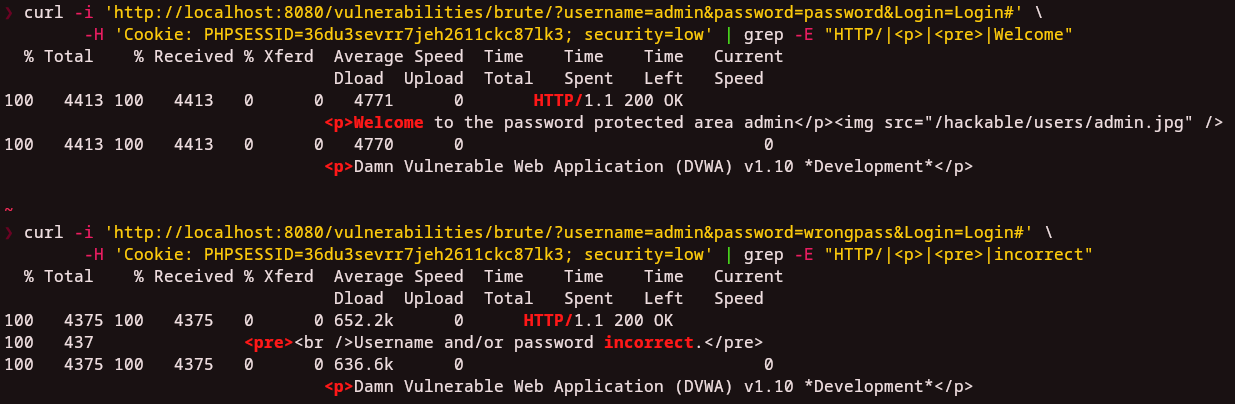
\includegraphics[width=0.9\linewidth]{imagenes/EvidenciaCurlTerminal.png}
    \caption{Ejecución de peticiones HTTP válidas e inválidas mediante cURL en la terminal.}
    \label{fig:curl_terminal}
\end{figure}

\subsection{Demuestra 4 diferencias (curl)}

A partir del análisis de los paquetes devueltos en la terminal mediante \texttt{cURL}, se identificaron cuatro diferencias estructurales y de contenido entre la respuesta de un acceso exitoso y uno fallido:

\begin{enumerate}
    \item \textbf{Mensaje de estado y validación en el cuerpo HTML:} 
    La diferencia más directa se encuentra en las etiquetas de texto devueltas. En la petición válida, el servidor responde con la etiqueta \texttt{<p>Welcome to the password protected area admin</p>}. En contraste, la petición inválida retorna el bloque \texttt{<pre>Username and/or password incorrect.</pre>}.

    \item \textbf{Tamaño total de la respuesta (Content-Length):} 
    Al analizar la transferencia de datos en la terminal, se observa que la respuesta del acceso válido transfiere un volumen superior de bytes (4,413 bytes) en comparación con el acceso fallido (4,375 bytes). Esta variación se debe a los elementos adicionales renderizados en la vista de bienvenida.

    \item \textbf{Carga del recurso de imagen de perfil (Avatar):} 
    La respuesta HTML correspondiente al acceso correcto incluye la etiqueta \texttt{<img src="/hackable/users/admin.jpg" />} para desplegar la imagen de perfil asignada al usuario \texttt{admin}. En la respuesta del acceso inválido, esta referencia a la imagen no existe.

    \item \textbf{Estructura del formulario y estado de la sesión en el DOM:} 
    En el acceso fallido, el servidor vuelve a renderizar el formulario de entrada (\texttt{<form action="\#">}) con sus campos de texto e instrucción de reintento. En el acceso exitoso, la estructura del formulario se omite o cambia su estado mostrando la bienvenida al área protegida.
\end{enumerate}

\subsection{Instalación y versión a utilizar (hydra)}

Para llevar a cabo las pruebas de fuerza bruta desde la línea de comandos mediante una herramienta multihilo optimizada, se procedió a instalar la suite \textit{THC-Hydra} a través del gestor de paquetes oficial del sistema operativo mediante el comando \texttt{sudo pacman -S hydra}.

Una vez completada la instalación, se verificó la disponibilidad de la herramienta y la versión instalada en el sistema mediante la ejecución del comando \texttt{hydra -v}. Como se evidencia en la Figura~\ref{fig:hydra_version}, la versión activa asignada para las ejecuciones del laboratorio corresponde a \textbf{Hydra v9.7}.

\begin{figure}[H]
    \centering
    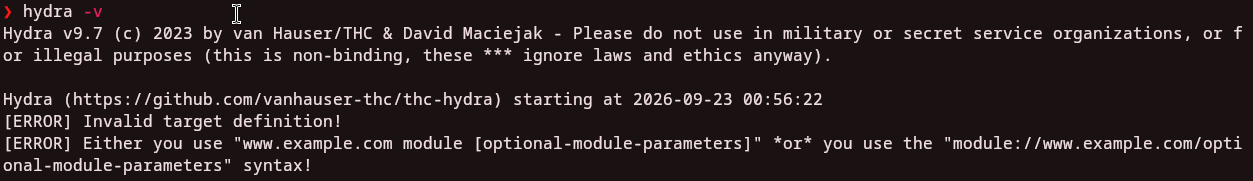
\includegraphics[width=0.9\linewidth]{imagenes/EvidenciaHydraVersion.png}
    \caption{Verificación en consola de la instalación y versión activa de Hydra (v9.7).}
    \label{fig:hydra_version}
\end{figure}

\subsection{Explicación de comando a utilizar (hydra)}

Para realizar el ataque de fuerza bruta sobre el formulario de autenticación de DVWA (bajo el nivel de seguridad \textit{low}), se empleó la herramienta \texttt{Hydra} utilizando su módulo especializado para formularios web por método GET (\texttt{http-get-form}).\\

El comando ejecutado con éxito en la terminal es el siguiente:

\begin{lstlisting}[breaklines=true, basicstyle=\ttfamily\small, frame=single]
hydra -L usuarios.txt -P passwords.txt localhost -s 8080 http-get-form '/vulnerabilities/brute/:username=^USER^&password=^PASS^&Login=Login:H=Cookie\:PHPSESSID=q1ttmlnqr44qp11mp75jefnm56; security=low:F=Username and/or password incorrect'
\end{lstlisting}

En la Figura~\ref{fig:hydra_execution} se evidencia la ejecución exitosa de la instrucción, la cual procesó las combinaciones de diccionarios y obtuvo los dos pares de credenciales válidos sin arrojar falsos positivos.\\

A continuación, se detalla la función de cada parámetro y bloque utilizado en la instrucción:
\begin{itemize}
    \item \textbf{\texttt{-L usuarios.txt}}: Archivo de texto que contiene el listado de nombres de usuario a evaluar en el ataque.
    \item \textbf{\texttt{-P passwords.txt}}: Archivo que contiene el diccionario de contraseñas candidatas.
    \item \textbf{\texttt{localhost -s 8080}}: Dirección IP o host objetivo y puerto expuesto por el contenedor de Docker donde corre la instancia de DVWA.
    \item \textbf{\texttt{http-get-form}}: Módulo de Hydra optimizado para interactuar con formularios web y mapear las respuestas del servidor.
    \item \textbf{\texttt{/vulnerabilities/brute/...}}: Estructura de la ruta y campos del formulario (\texttt{username}, \texttt{password} y el botón \texttt{Login}), haciendo uso de los comodines \textbf{\texttt{\^USER\^}} y \textbf{\texttt{\^PASS\^}} para la iteración de los diccionarios.
    \item \textbf{\texttt{H=Cookie\textbackslash{}:PHPSESSID=...}}: Cabecera HTTP personalizada que inyecta la cookie de sesión activa y el nivel de seguridad (\textit{security=low}), evitando la expiración de sesión y las redirecciones a la pantalla de login.
    \item \textbf{\texttt{F=Username and/or password incorrect}}: Cadena de control ubicada al final de la estructura que permite al analizador de Hydra identificar los intentos fallidos y descartar falsos positivos, aislando únicamente las credenciales correctas.
\end{itemize}

\begin{figure}[H]
    \centering
    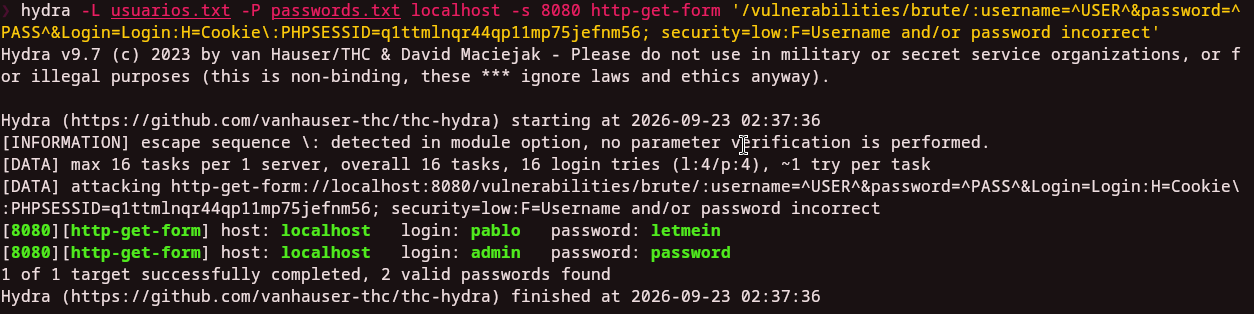
\includegraphics[width=0.9\linewidth]{imagenes/Evidencia_hydra.png}
    \caption{Evidencia de la ejecución exitosa de Hydra mostrando las 2 credenciales válidas encontradas.}
    \label{fig:hydra_execution}
\end{figure}

\subsection{Obtención de al menos 2 pares (hydra)}

Una vez ejecutado el comando de fuerza bruta con la configuración optimizada para la versión 9.7 de \texttt{Hydra}, la herramienta procesó todas las combinaciones posibles entre los usuarios definidos en el archivo \texttt{usuarios.txt} y las contraseñas del diccionario \texttt{passwords.txt}.\\

Gracias al uso correcto de la cabecera de sesión y la cadena de control de fallo ubicada al final de la instrucción, el analizador interno de Hydra descartó los falsos positivos derivados de las redirecciones y evaluó únicamente las respuestas legítimas del servidor web en el contenedor de Docker. Como se observa en la Figura~\ref{fig:hydra_execution}, la ejecución concluyó de forma exitosa indicando la localización de dos credenciales válidas.

A partir de la salida en consola de la herramienta, se obtuvieron de manera automatizada los siguientes dos pares válidos de usuario y contraseña:
\begin{itemize}
    \item \textbf{Par 1:} \texttt{admin} : \texttt{password}
    \item \textbf{Par 2:} \texttt{pablo} : \texttt{letmein}
\end{itemize}

\subsection{Explicación paquete curl (tráfico)}

A partir de la captura de tráfico realizada en Wireshark sobre la interfaz de red \textit{loopback} (\texttt{lo}), se analizó el paquete HTTP generado tras la ejecución de la instrucción \texttt{cURL} en la terminal. 

En la inspección detallada de la trama a nivel de aplicación mostrada en la Figura~\ref{fig:trafico_curl}, se identifican las siguientes características clave:
\begin{itemize}
    \item \textbf{Cabecera \texttt{User-Agent}}: Se observa de forma explícita la firma \texttt{User-Agent: curl/8.22.0}, lo cual corrobora de manera inequívoca que la petición proviene de la herramienta nativa \texttt{cURL} y no de un navegador web convencional.
    \item \textbf{Estructura de la Solicitud GET}: La URI transporta los parámetros del formulario de autenticación en texto plano (\texttt{username=admin\&password=password\&Login=Login}), acompañados de la cabecera de sesión y el nivel de seguridad correspondientes.
    \item \textbf{Comportamiento a nivel de transporte}: Al ser una ejecución individual desde la consola, el flujo TCP se restringe a una única conexión limpia, secuencial y de corta duración (apertura del socket, envío de la petición, recepción de la respuesta y cierre inmediato).
\end{itemize}

\begin{figure}[H]
    \centering
    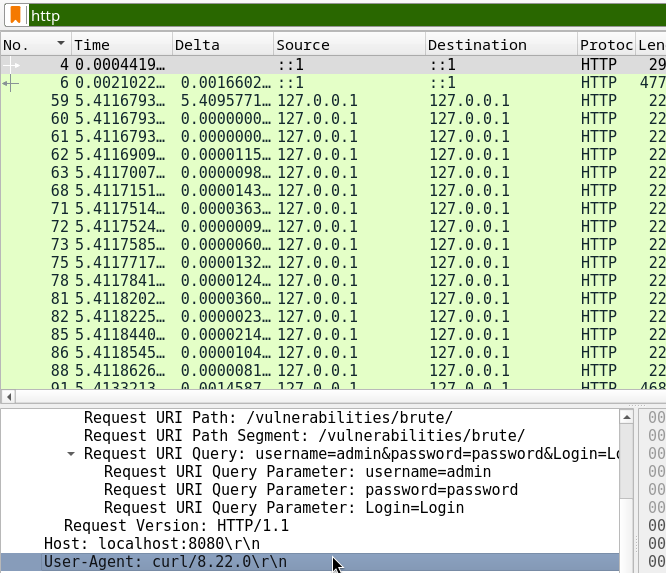
\includegraphics[width=0.75\linewidth]{imagenes/EvidenciaTráficoCurl.png}
    \caption{Captura en Wireshark del paquete HTTP generado mediante cURL, destacando la cabecera \textit{User-Agent} y los parámetros de consulta.}
    \label{fig:trafico_curl}
\end{figure}

\subsection{Explicación paquete burp (tráfico)}

A partir del análisis del tráfico capturado en Wireshark durante la ejecución de ataques automatizados mediante \textit{Burp Suite Intruder}, se observa un flujo de peticiones estructurado y característico. 

Al inspeccionar las tramas correspondientes en la capa de aplicación presentadas en la Figura~\ref{fig:trafico_burp}, se identifican los siguientes elementos distintivos:
\begin{itemize}
    \item \textbf{Cabecera \texttt{User-Agent}}: A diferencia de las herramientas de línea de comandos, el tráfico generado a través de Burp Suite conserva la firma del navegador web utilizado para la sesión (por ejemplo, \texttt{Mozilla/5.0 (X11; Linux x86\_64)...}), simulando peticiones legítimas de un cliente web convencional.
    \item \textbf{Estructura de peticiones por lotes}: En la lista de paquetes se aprecia la secuencia iterativa generada por el módulo \textit{Intruder} evaluando los diferentes parámetros de los diccionarios (\texttt{username=test}, \texttt{admin}, \texttt{pablo}, entre otros).
    \item \textbf{Comportamiento de la conexión}: Las peticiones muestran el uso de cabeceras de control y gestión de estado asociadas al navegador, permitiendo reenviar y modificar dinámicamente el tráfico hacia el contenedor local de DVWA.
\end{itemize}

\begin{figure}[H]
    \centering
    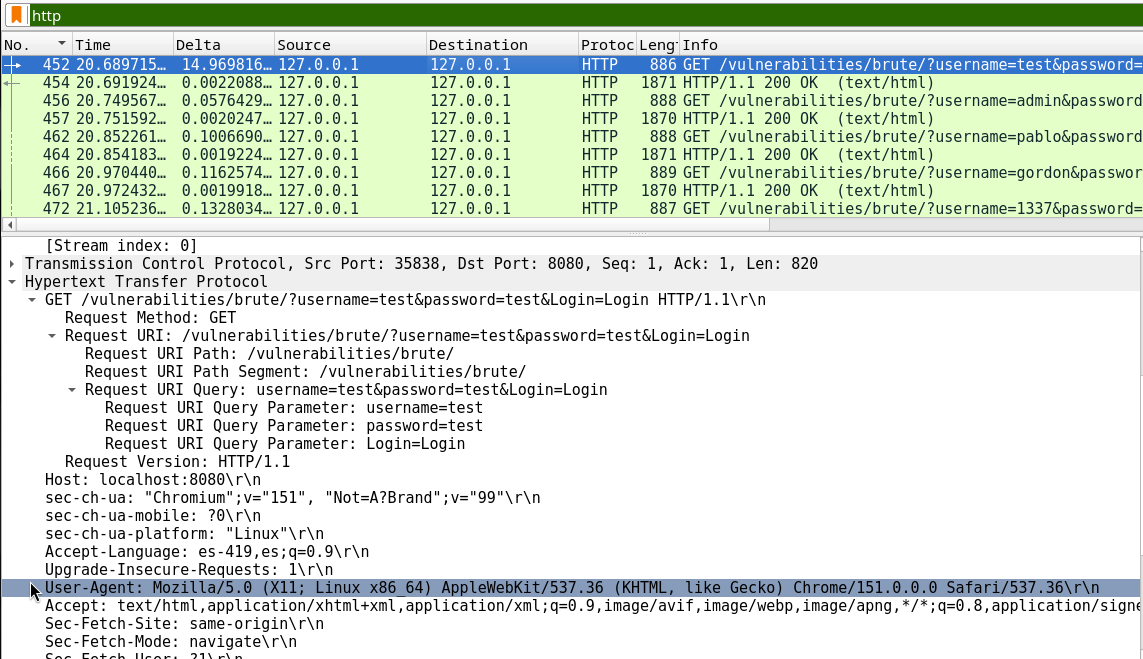
\includegraphics[width=0.9\linewidth]{imagenes/EvidenciaTráficoBurp.png}
    \caption{Captura en Wireshark del tráfico generado por Burp Suite Intruder, destacando la cabecera \textit{User-Agent} del navegador y la secuencia de peticiones.}
    \label{fig:trafico_burp}
\end{figure}

\subsection{Explicación paquete hydra (tráfico)}

A partir del análisis de la captura de tráfico en Wireshark durante la ejecución de \textit{Hydra}, el flujo de red se distingue por una alta concurrencia y un paralelismo masivo de peticiones. 

Al inspeccionar los paquetes capturados a nivel de aplicación y transporte ilustrados en la Figura~\ref{fig:trafico_hydra}, se destacan las siguientes características técnicas:
\begin{itemize}
    \item \textbf{Cabecera \texttt{User-Agent}}: La herramienta presenta una firma específica, reflejada en la traza como \texttt{User-Agent: Mozilla/5.0 (Hydra)}, la cual delata de forma inequívoca el uso de esta herramienta de ataque automatizado.
    \item \textbf{Alta Concurrencia y Tiempos (\textit{Delta})}: En la lista de paquetes se observa una ráfaga simultánea de solicitudes con tiempos de diferencia (\textit{Delta}) de \texttt{0.000000} segundos o fracciones mínimas, evidenciando el comportamiento multihilo enfocado en saturar el servicio.
    \item \textbf{Comportamiento de red}: A diferencia de las ejecuciones secuenciales o controladas por lotes anteriores, Hydra genera múltiples aperturas de conexiones independientes de manera simultánea hacia el puerto \texttt{8080} del contenedor Docker.
\end{itemize}

\begin{figure}[H]
    \centering
    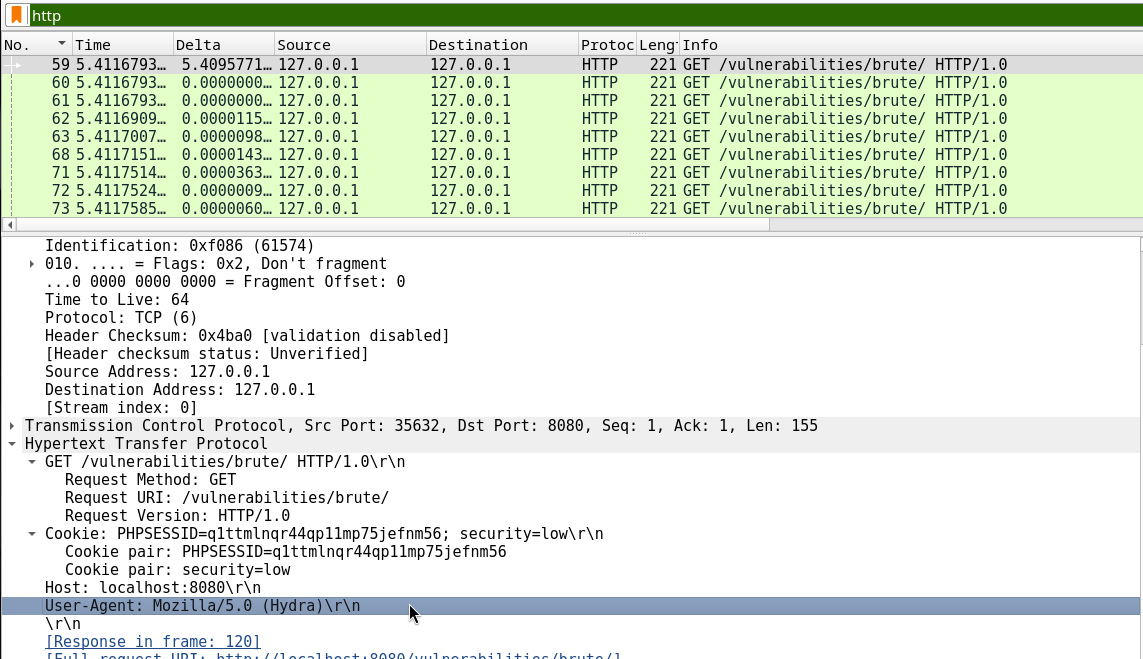
\includegraphics[width=0.9\linewidth]{imagenes/EvidenciaTráficoHydra.png}
    \caption{Captura en Wireshark del tráfico masivo y concurrente generado por Hydra, mostrando la cabecera \textit{User-Agent} y los tiempos Delta mínimos.}
    \label{fig:trafico_hydra}
\end{figure}

\newpage

\subsection{Mención de las diferencias (tráfico)}

A partir del análisis individual y la contrastación de las trazas de red capturadas en Wireshark (ver Figuras \ref{fig:trafico_curl}, \ref{fig:trafico_burp} y \ref{fig:trafico_hydra}), es posible establecer claras diferencias empíricas en el comportamiento, la firma y el patrón de comunicación de las tres herramientas evaluadas contra el servidor local de DVWA:

\begin{itemize}
    \item \textbf{Firma del cliente (\textit{User-Agent})}: Como se evidencia en las tramas HTTP interceptadas, \texttt{cURL} se identifica de forma transparente con su versión (\texttt{curl/8.22.0}); \textbf{Burp Suite} enmascara el ataque camuflando las peticiones bajo la firma de un navegador web convencional (ej. \textit{Chromium/Mozilla}); y \textbf{Hydra} presenta una identificación explícita de herramienta automatizada (ej. \textit{Mozilla/5.0 (Hydra)}).
    \item \textbf{Patrón de concurrencia y tiempos (\textit{Delta})}: Las métricas temporales de Wireshark demuestran que \texttt{cURL} opera mediante un flujo estrictamente secuencial; \textbf{Burp Suite Intruder} ejecuta peticiones automatizadas por lotes de forma controlada; en contraste, \textbf{Hydra} genera una ráfaga masiva e inmediata con tiempos \textit{Delta} de valor cero, evidenciando un ataque multihilo agresivo.
    \item \textbf{Gestión de conexiones (Capa de Transporte)}: Las trazas de sockets muestran que \texttt{cURL} abre y cierra una conexión TCP por cada consulta. \textbf{Burp Suite} optimiza el flujo reutilizando conexiones persistentes, mientras que \textbf{Hydra} abre múltiples sockets independientes en paralelo contra el puerto \texttt{8080} del contenedor.
\end{itemize}

\subsection{Detección de SW (tráfico)}

Basándose en la inspección detallada de los paquetes de red capturados en Wireshark (ver Figuras \ref{fig:trafico_curl}, \ref{fig:trafico_burp} y \ref{fig:trafico_hydra}), los sistemas de defensa perimetral pueden realizar una detección efectiva de software (\textit{Software Detection}) respaldada por los siguientes indicadores empíricos:

\begin{itemize}
    \item \textbf{Detección del cliente por firmas estáticas}: Las trazas de red permiten identificar herramientas ofensivas según su cabecera \texttt{User-Agent} (evidenciadas en las capturas previas). Mientras que \texttt{cURL} y \texttt{Hydra} delatan su presencia de forma directa con firmas inequívocas (\textit{curl/...} y \textit{Mozilla/5.0 (Hydra)}), \textbf{Burp Suite} elude la detección por firma estática al camuflarse con el agente de un navegador real, requiriendo un análisis dinámico.
    \item \textbf{Detección por patrones de comportamiento y tráfico}: La evidencia temporal registrada en Wireshark muestra que los ataques automatizados dejan huellas de red inconfundibles. Las solicitudes masivas y concurrentes con tiempos \textit{Delta} mínimos de \textbf{Hydra} delatan un ataque por saturación; los lotes estructurados de \textbf{Burp Suite} evidencian automatización controlada; y el flujo espaciado de \texttt{cURL} refleja un uso secuencial.
    \item \textbf{Detección de tecnologías del servidor}: Analizando los campos de respuesta HTTP devueltos por el servidor (registrados en las mismas trazas de las herramientas anteriores), se pueden extraer metadatos técnicos en cabeceras como \texttt{Server} (ej. Apache) o \texttt{X-Powered-By} (ej. PHP), mapeando la infraestructura expuesta en el contenedor de Docker.
\end{itemize}

\subsection{Interacción con el formulario (python)}

Para automatizar el proceso de fuerza bruta sobre el formulario de autenticación de DVWA, se desarrolló un script en \textbf{Python} utilizando la librería \texttt{requests}. El script interactúa directamente con la ruta vulnerable mediante peticiones HTTP GET, evaluando de forma masiva combinaciones de nombres de usuario y contraseñas.

Como se detalla en la \textbf{Figura \ref{fig:script_python}}, la ejecución de este script en la terminal permite observar de forma empírica el flujo del ataque: muestra el mensaje de inicialización de la sesión con las cookies activas, el procesamiento secuencial del espacio de búsqueda de 70 combinaciones, y la detección en tiempo real de los aciertos válidos (como \texttt{admin:password}, \texttt{pablo:letmein}, etc.) junto al rendimiento operativo de \textbf{407.71 intentos por segundo}.

\begin{figure}[H]
    \centering
    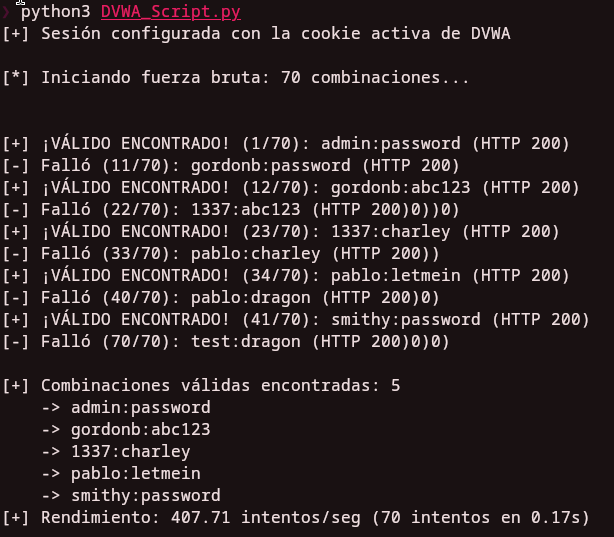
\includegraphics[width=0.7\linewidth]{imagenes/EvidenciaScriptPython.png}
    \caption{Ejecución del script en Python, mostrando en consola la detección exitosa de credenciales válidas y las métricas de rendimiento.}
    \label{fig:script_python}
\end{figure}

\newpage

A continuación se presenta el código fuente implementado, el cual refleja la lógica de inyección de sesión y validación descrita en la evidencia gráfica anterior:

\begin{lstlisting}[language=Python, breaklines=true, basicstyle=\ttfamily\small, frame=single, showspaces=false, showstringspaces=false]
#!/usr/bin/env python3
"""
Brute force contra DVWA (vulnerabilities/brute)
Uso educativo - Laboratorio de Criptografia y Seguridad en redes
"""

import itertools
import time
import requests

# --- Configuracion ---
BASE_URL = "http://localhost:8080"
BRUTE_URL = f"{BASE_URL}/vulnerabilities/brute/"

# Diccionarios de prueba
USERS = ["admin", "gordonb", "1337", "pablo", "smithy", "root", "test"]
PASSWORDS = [
    "password",
    "abc123",
    "charley",
    "letmein",
    "123456",
    "admin",
    "qwerty",
    "111111",
    "iloveyou",
    "dragon",
]


def obtener_sesion():
  """Inyecta directamente la cookie de sesion activa y el nivel de seguridad
  para asegurar el acceso al modulo vulnerable.
  """
  s = requests.Session()

  # Cookie extraida de sesion activa
  s.cookies.set("PHPSESSID", "q1ttmlnqr44qp11mp75jefnm56")
  s.cookies.set("security", "low")

  print("[+] Sesion configurada con la cookie activa de DVWA")
  return s


def intento_login(session, usuario, password):
  """Realiza un intento de login contra vulnerabilities/brute utilizando parametros GET.
  """
  params = {"username": usuario, "password": password, "Login": "Login"}

  r = session.get(BRUTE_URL, params=params, timeout=10)

  # Si el mensaje de error clasico NO esta presente, las credenciales son correctas
  if "Username and/or password incorrect" not in r.text:
    return True, r
  return False, r


def main():
  session = obtener_sesion()
  encontrados = []
  total = len(USERS) * len(PASSWORDS)
  inicio = time.time()
  intentos = 0

  print(f"\n[*] Iniciando fuerza bruta: {total} combinaciones...\n")

  for usuario, password in itertools.product(USERS, PASSWORDS):
    intentos += 1
    exito, resp = intento_login(session, usuario, password)

    if exito:
      print(
          f"\n[+] ¡VALIDO ENCONTRADO! ({intentos}/{total}): {usuario}:{password}"
          f" (HTTP {resp.status_code})"
      )
      encontrados.append((usuario, password))
    else:
      print(
          f"[-] Fallo ({intentos}/{total}): {usuario}:{password}"
          f" (HTTP {resp.status_code})",
          end="\r",
      )

  duracion = time.time() - inicio
  print(f"\n\n[+] Combinaciones validas encontradas: {len(encontrados)}")
  for u, p in encontrados:
    print(f"    -> {u}:{p}")
  print(
      f"[+] Rendimiento: {intentos/duracion:.2f} intentos/seg "
      f"({intentos} intentos en {duracion:.2f}s)"
  )


if __name__ == "__main__":
  main()
\end{lstlisting}

Los componentes principales del script que explican los resultados visualizados en la figura son:
\begin{itemize}
    \item \textbf{Gestión de Sesión}: Utiliza \texttt{requests.Session()} para fijar las cookies de control (\texttt{PHPSESSID} y el nivel de seguridad \texttt{security=low}).
    \item \textbf{Generación de Combinaciones}: Emplea \texttt{itertools.product} para recorrer eficientemente el producto cartesiano entre las listas de usuarios y claves.
    \item \textbf{Validación de Respuesta}: Evalúa el cuerpo HTML devuelto por el servidor buscando la ausencia de la cadena de error oficial para descartar falsos positivos.
\end{itemize}

\newpage

\subsection{Cabeceras HTTP (python)}

Durante la ejecución del script en Python utilizando la librería \texttt{requests}, cada petición HTTP enviada hacia el contenedor de DVWA incorpora cabeceras de control esenciales para direccionar la solicitud, mantener el estado de la sesión y estructurar el ataque.

Como se evidencia en la captura de tráfico de Wireshark de la \textbf{Figura \ref{fig:cabeceras_python}}, la inspección de los paquetes sobre la interfaz de red permite identificar con precisión los campos y parámetros transmitidos por el script:

\begin{figure}[H]
    \centering
    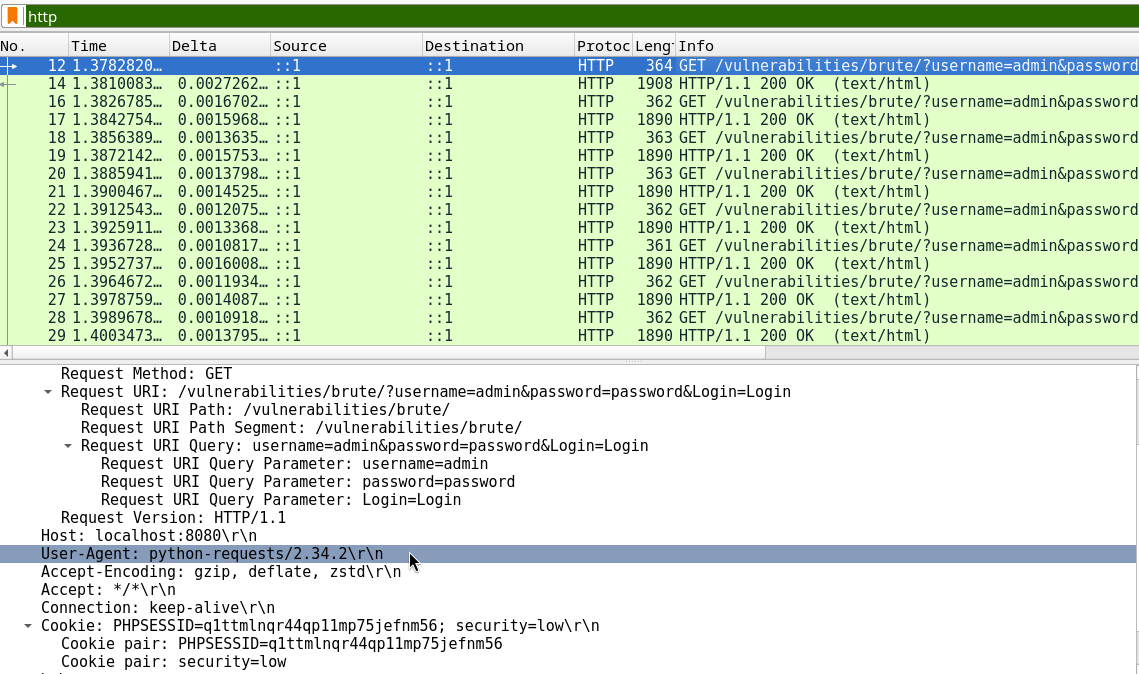
\includegraphics[width=0.9\linewidth]{imagenes/EvidenciaCabecerasPython.png}
    \caption{Captura de Wireshark mostrando las cabeceras HTTP y los parámetros GET enviados por la librería \texttt{requests}.}
    \label{fig:cabeceras_python}
\end{figure}

Las cabeceras y elementos clave observados en la traza son los siguientes:
\begin{itemize}
    \item \textbf{Cabecera \texttt{Cookie}}: Transporta explícitamente los valores de control \texttt{PHPSESSID} (para mantener una sesión activa y autorizada) y \texttt{security=low} (para asegurar que el servidor mantenga el nivel de seguridad bajo durante las pruebas).
    \item \textbf{Cabecera \texttt{Host}}: Define el dominio y el puerto de destino de la aplicación (\texttt{localhost:8080}), permitiendo que el contenedor Docker enrute de forma adecuada la consulta.
    \item \textbf{Cabecera \texttt{User-Agent}}: Identifica el software cliente responsable de la petición. En la traza se aprecia claramente la firma característica de la librería (\texttt{python-requests/2.34.2}), la cual delata de inmediato el uso de un script automatizado frente a un navegador web tradicional.
    \item \textbf{Parámetros de la URL (\textit{Query String})}: En la línea de solicitud GET, el script adjunta dinámicamente las variables correspondientes al formulario vulnerable (\texttt{username}, \texttt{password} y \texttt{Login=Login}).
\end{itemize}

\subsection{Obtención de al menos 2 pares (python)}

Tras la ejecución automatizada del script de fuerza bruta contra el formulario de autenticación del módulo de vulnerabilidades de DVWA, el sistema procesó con éxito el espacio de búsqueda completo compuesto por los diccionarios de usuarios y contraseñas.

Como se visualiza en la evidencia de ejecución de la \textbf{Figura \ref{fig:script_python}}, el algoritmo logró identificar de manera completamente automatizada múltiples credenciales legítimas. El script diferenció con precisión los intentos fallidos de los aciertos válidos mediante la validación de la respuesta HTTP, obteniendo con éxito los siguientes pares de usuario y contraseña:

\begin{itemize}
    \item \textbf{\texttt{admin:password}}: Validado correctamente en el primer intento del conjunto de pruebas, devolviendo un código HTTP 200 sin el mensaje de error restrictivo.
    \item \textbf{\texttt{pablo:letmein}}: Identificado de forma precisa dentro del subconjunto de combinaciones del usuario \textit{pablo}.
    \item \textbf{Credenciales adicionales detectadas}: De manera complementaria, el script también extrajo con éxito los pares \texttt{gordonb:abc123}, \texttt{1337:charley} y \texttt{smithy:password}, demostrando la exhaustividad de la prueba.
\end{itemize}

Estos resultados confirman la total funcionalidad del desarrollo en Python, logrando validar las credenciales del sistema en un tiempo de ejecución sumamente eficiente de 0.17 segundos para el total de las 70 combinaciones evaluadas.

\subsection{Comparación de rendimiento con Hydra, Burpsuite, y cURL (python)}

La evaluación comparativa entre el script en Python desarrollado y las herramientas especializadas (\textbf{Hydra}, \textbf{Burp Suite} y \textbf{cURL}) permite contrastar el desempeño bajo dos ejes fundamentales: la velocidad de procesamiento (rendimiento operativo) y la facilidad de detección por parte de los mecanismos de seguridad perimetral.

\begin{itemize}
    \item \textbf{Rendimiento y Velocidad de Procesamiento}:
    \begin{itemize}
        \item \textbf{Hydra}: Se posiciona como la herramienta más rápida del análisis debido a su desarrollo nativo en C y su arquitectura fuertemente paralelizada (multihilo), diseñada específicamente para ráfagas masivas de fuerza bruta.
        \item \textbf{Python (\texttt{requests})}: Demostró un rendimiento sumamente eficiente en entornos locales. Mediante la reutilización de conexiones y el mantenimiento de sesión con \texttt{requests.Session()}, el script alcanzó una velocidad de \textbf{407.71 intentos por segundo}, procesando el espacio completo de 70 combinaciones en tan solo 0.17 segundos. Esto supera ampliamente el rendimiento de ejecuciones secuenciales o manuales.
        \item \textbf{Burp Suite (Intruder)}: Su velocidad de ejecución se encuentra moderada por la sobrecarga de su interfaz gráfica y las políticas de control de concurrencia del motor, aunque optimiza el envío mediante conexiones persistentes (\textit{Keep-Alive}).
        \item \textbf{cURL}: Presenta el rendimiento operativo más bajo para pruebas masivas, ya que opera de forma estrictamente secuencial y genera un cuello de botella debido al coste de abrir y cerrar un socket TCP independiente por cada consulta HTTP.
    \end{itemize}
    
    \item \textbf{Detección y Huella en la Red}:
    \begin{itemize}
        \item \textbf{Hydra y cURL}: Facilitan enormemente la labor defensiva al dejar huellas estáticas inequívocas en las cabeceras \texttt{User-Agent} (\texttt{Mozilla/5.0 (Hydra)} y \texttt{curl/8.22.0}), permitiendo reglas de bloqueo directo en sistemas WAF.
        \item \textbf{Python}: Aunque ofrece total flexibilidad para modificar el código, la librería \texttt{requests} expone por defecto su propia firma (\texttt{python-requests/x.xx.x}), lo que delata inmediatamente el uso de un script automatizado a menos que se implemente la suplantación manual de cabeceras (\textit{spoofing}).
        \item \textbf{Burp Suite}: Destaca como la herramienta con mayor capacidad de evasión por firma estática, ya que reenvía las solicitudes camufladas bajo la identidad de un navegador web convencional, obligando a los sistemas de defensa a depender de análisis heurísticos basados en tiempos \textit{Delta} y patrones de tráfico.
    \end{itemize}
\end{itemize}

\newpage
\subsection{Demuestra 4 métodos de mitigación (investigación)}

Para contrarrestar y prevenir ataques de fuerza bruta en aplicaciones web, es fundamental implementar una estrategia de defensa en profundidad. A continuación, se describen cuatro de los métodos de mitigación más comunes y eficaces en la industria:

\begin{itemize}
    \item \textbf{1. Limitación de Tasa (\textit{Rate Limiting} o \textit{Throttling})}
    \begin{itemize}
        \item \textbf{Funcionamiento}: Restringe el número máximo de peticiones HTTP permitidas desde una misma dirección IP o sesión en una ventana de tiempo determinada (ej. bloquear o retrasar peticiones si se superan los 5 intentos por minuto). Cuando se excede el límite, el servidor responde típicamente con un código de estado \texttt{HTTP 429 Too Many Requests}.
        \item \textbf{Escenario de mayor eficacia}: Es altamente eficaz para frenar ataques automatizados masivos y de alta concurrencia (como los ejecutados mediante \textit{Hydra} o como el script desarrollado en \textit{Python}), ya que neutraliza la velocidad del atacante s的时 saturar el servicio.
    \end{itemize}

    \item \textbf{2. Bloqueo Temporal de Cuenta (\textit{Account Lockout})}
    \begin{itemize}
        \item \textbf{Funcionamiento}: Desactiva temporalmente el acceso a una cuenta de usuario específica tras alcanzar un umbral predefinido de intentos fallidos consecutivos (por ejemplo, 5 o 10 errores). La cuenta se bloquea por un tiempo determinado o requiere una verificación adicional (como un correo de desbloqueo).
        \item \textbf{Escenario de mayor eficacia}: Es idóneo para mitigar ataques de fuerza bruta dirigidos o ataques de relleno de credenciales (\textit{credential stuffing}) contra cuentas concretas, impidiendo que un script pruebe miles de combinaciones de contraseñas de forma indefinida sobre un mismo usuario.
    \end{itemize}

    \item \textbf{3. Desafíos Interactivos (\textit{CAPTCHA} o Pruebas de Desafío)}
    \begin{itemize}
        \item \textbf{Funcionamiento}: Introduce un mecanismo de validación visual, lógico o basado en comportamiento (como reCAPTCHA, hCaptcha o sistemas invisibles de análisis de riesgo) que resulta sencillo de resolver para un usuario humano pero computacionalmente complejo para un script automatizado.
        \item \textbf{Escenario de mayor eficacia}: Es muy eficaz en formularios públicos de autenticación, recuperación de contraseñas y registro, impidiendo que herramientas como \textit{cURL}, \textit{Burp Suite} o scripts personalizados interactúen masivamente con el formulario sin la intervención humana.
    \end{itemize}

    \item \textbf{4. Autenticación Multifactor (MFA / 2FA)}
    \begin{itemize}
        \item \textbf{Funcionamiento}: Exige al usuario proporcionar una evidencia de identidad adicional y desacoplada de la contraseña tradicional, como un código temporal de un solo uso (TOTP) generado por una aplicación autenticadora, notificaciones push o llaves de seguridad físicas (FIDO2/WebAuthn).
        \item \textbf{Escenario de mayor eficacia}: Representa la barrera de defensa definitiva contra ataques de fuerza bruta y robo de credenciales. Su eficacia radica en que, incluso si el atacante logra adivinar o vulnerar la contraseña mediante fuerza bruta, el acceso al sistema es denegado al carecer del segundo factor dinámico o físico.
    \end{itemize}
\end{itemize}

% Please add the following required packages to your document preamble:
%\begin{table}[htbp]

\section*{Conclusiones y comentarios}
\addcontentsline{toc}{section}{Conclusiones y comentarios}

A partir de las actividades prácticas desarrolladas en el laboratorio sobre la plataforma vulnerable DVWA, se presentan las siguientes conclusiones técnicas y comentarios reflexivos:

\begin{itemize}
    \item \textbf{Eficacia del ataque de fuerza bruta frente a mecanismos de autenticación débiles:} 
    La experiencia práctica demostró que la autenticación basada únicamente en credenciales estáticas (usuario/contraseña) sin controles de tasa de peticiones (\textit{rate limiting}) es altamente vulnerable a la automatización. Todas las herramientas evaluadas (Burp Suite, Hydra, cURL y el script en Python) lograron identificar exitosamente las credenciales válidas (\texttt{admin:password} y \texttt{pablo:letmein}) en cuestión de segundos o milisegundos.

    \item \textbf{Compromiso entre velocidad de ejecución y capacidad de evasión:} 
    Existe una relación inversa entre la rapidez del ataque y su invisibilidad ante sistemas defensivos (WAF/IDS/IPS):
    \begin{itemize}
        \item \textbf{Hydra} y el script en \textbf{Python} destacaron por su alto rendimiento operativo (alcanzando más de 400 intentos/seg en local), pero generan ráfagas de tráfico masivo con tiempos \textit{Delta} mínimos y cabeceras \texttt{User-Agent} delatadoras (\texttt{Hydra}, \texttt{python-requests}), siendo fácilmente detectables y bloqueables.
        \item \textbf{Burp Suite Intruder} ofreció el mayor nivel de evasión por firma estática al camuflar el tráfico bajo el \texttt{User-Agent} de un navegador legítimo, aunque a costa de una menor velocidad de inyección.
        \item \textbf{cURL} demostró ser ideal para la inspección y replicación puntual de solicitudes desde la línea de comandos, pero resulta ineficiente para ataques masivos debido al cuello de botella que implica abrir y cerrar sockets TCP de forma secuencial.
    \end{itemize}

    \item \textbf{Relevancia del análisis de tráfico y firmas en capas de red y aplicación:} 
    La inspección realizada con Wireshark evidenció que ningún ataque automatizado es completamente transparente. Incluso cuando se suplanta la identidad del cliente (\textit{User-Agent spoofing}), los patrones comportamentales —tales como la frecuencia de peticiones, la reutilización de la misma cookie de sesión en paralelo y la falta de carga de recursos estáticos secundarios (CSS, JS, imágenes)— permiten a los analizadores heurísticos e IDSs catalogar el tráfico como malicioso.

    \item \textbf{Importancia de la defensa en profundidad:} 
    Ningún método de mitigación es suficiente por sí solo. Para proteger adecuadamente los endpoints de autenticación en entornos de producción, es imprescindible implementar un enfoque multicapa que combine \textbf{Rate Limiting} en el WAF/reverse proxy, \textbf{Bloqueo Temporal de Cuentas} a nivel de lógica de negocio, \textbf{CAPTCHA contextual} ante anomalías de tráfico y, de manera fundamental, \textbf{Autenticación Multifactor (MFA)}, la cual invalida el impacto de una contraseña comprometida mediante fuerza bruta.
\end{itemize}

\end{document}
